% !TEX program = xelatex
\documentclass[11pt,a4paper]{article}
\newcommand{\DOCFOOT}{AMPERE POINT · Q11 with a Shelly X module · test documentation v1 · 28 September 2026}
% Wspólna preambuła dokumentów dla producenta (xelatex); kopia z raportu DLB, czcionki systemowe Windows
\usepackage{fontspec}
% \ZHDOC zdefiniowane przed \input => cały dokument po chińsku (Noto Sans CJK SC + łamanie wierszy CJK)
\ifdefined\ZHDOC
  \setmainfont{Microsoft YaHei}[Scale=0.90]
  \setsansfont{Microsoft YaHei}[Scale=0.90]
  \XeTeXlinebreaklocale "zh"
  \XeTeXlinebreakskip = 0pt plus 1pt minus 0.1pt
\else
  \setmainfont{Calibri}
  \setsansfont{Calibri}
\fi
\setmonofont{Consolas}[Scale=0.86]
\newfontfamily\cjkfont{Microsoft YaHei}[Scale=0.90]
\newfontfamily\latinfont{Calibri}
\newcommand{\pl}[1]{{\latinfont #1}}
\usepackage[a4paper,top=2.0cm,bottom=2.0cm,left=1.9cm,right=1.9cm]{geometry}
\usepackage{graphicx}
\usepackage[table]{xcolor}
\usepackage{booktabs,longtable,array,tabularx,enumitem,fancyhdr,caption}
\usepackage[most]{tcolorbox}
\usepackage[hidelinks,unicode]{hyperref}
\usepackage{needspace}
\usepackage{float}
\emergencystretch=2.5em
\setlength{\parindent}{0pt}\setlength{\parskip}{5pt}
\renewcommand{\arraystretch}{1.22}
\captionsetup{font=small,labelfont=bf,skip=3pt}
\setlist{nosep,leftmargin=*}
\setcounter{secnumdepth}{2}

\definecolor{apnavy}{HTML}{1A1A1A}
\definecolor{apink}{HTML}{1C2430}
\definecolor{apmuted}{HTML}{5B6675}
\definecolor{apline}{HTML}{E3E3E3}
\definecolor{apbg}{HTML}{F5F5F5}
\definecolor{apaccent}{HTML}{EC6434}
\definecolor{apaccentbg}{HTML}{FDEDE6}
\definecolor{apwarn}{HTML}{B9791B}
\definecolor{apwarnbg}{HTML}{FBF1DE}
\definecolor{apred}{HTML}{B91C1C}
\definecolor{apredbg}{HTML}{FEE2E2}
\definecolor{apgreen}{HTML}{1F8A4C}
\definecolor{apgreenbg}{HTML}{E7F5EC}
\definecolor{aphead}{HTML}{EDEDED}

\pagestyle{fancy}\fancyhf{}
\renewcommand{\headrulewidth}{0pt}
\fancyfoot[L]{\footnotesize\color{apmuted}\DOCFOOT}
\fancyfoot[R]{\footnotesize\color{apmuted}\thepage\,/\,\pageref{LastPage}}
\usepackage{lastpage}

\usepackage{titlesec}
\titleformat{\section}{\Large\bfseries\color{apnavy}}{\thesection}{0.6em}{}
\titlespacing*{\section}{0pt}{14pt}{6pt}
\titleformat{\subsection}{\large\bfseries\color{apnavy}}{\thesubsection}{0.6em}{}
\titlespacing*{\subsection}{0pt}{10pt}{4pt}

% pasek tytułowy
\newcommand{\apheader}[3]{%
\noindent
\includegraphics[height=1.0cm]{logo_ap.png}\hfill
\raisebox{0.25cm}{\parbox[t]{10.5cm}{\raggedleft\footnotesize\color{apmuted}#3}}\\[0.25cm]
{\color{apaccent}\rule{\textwidth}{1.8pt}}\\[0.30cm]
{\bfseries\color{apnavy}\LARGE #1}\\[0.18cm]
{\large\color{apmuted}#2}\\[0.2cm]}

% ramki
\newtcolorbox{apbox}[1][]{enhanced,breakable,colback=apbg,colframe=apline,boxrule=0.6pt,arc=3pt,left=7pt,right=7pt,top=5pt,bottom=5pt,fonttitle=\bfseries,coltitle=apnavy,colbacktitle=aphead,title={#1}}
\newtcolorbox{apwarnb}[1][]{enhanced,breakable,colback=apwarnbg,colframe=apwarn,boxrule=0.6pt,arc=3pt,left=7pt,right=7pt,top=5pt,bottom=5pt,fonttitle=\bfseries,title={#1}}
\newtcolorbox{apredb}[1][]{enhanced,breakable,colback=apredbg,colframe=apred,boxrule=0.6pt,arc=3pt,left=7pt,right=7pt,top=5pt,bottom=5pt,fonttitle=\bfseries,title={#1}}
\newtcolorbox{apgreenb}[1][]{enhanced,breakable,colback=apgreenbg,colframe=apgreen,boxrule=0.6pt,arc=3pt,left=7pt,right=7pt,top=5pt,bottom=5pt,fonttitle=\bfseries,title={#1}}

% komórka ze zrzutem ekranu: #1 szerokość, #2 plik, #3 podpis
\newcommand{\shot}[3]{%
\begin{minipage}[t]{#1}
  \vspace{0pt}\centering
  \includegraphics[width=\linewidth,height=6.2cm,keepaspectratio]{#2}\par\vspace{3pt}
  {\footnotesize\color{apink}#3\par}
\end{minipage}}


% mniejsza komórka ze zdjęciem (np. gniazda aut)
\newcommand{\shotsm}[3]{%
\begin{minipage}[t]{#1}
  \vspace{0pt}\centering
  \includegraphics[width=\linewidth,height=4.6cm,keepaspectratio]{#2}\par\vspace{3pt}
  {\footnotesize\color{apink}#3\par}
\end{minipage}}

\newcommand{\kroknum}[1]{{\colorbox{apaccent}{\textcolor{white}{\bfseries\small\,#1\,}}}}
\newcommand{\dpn}[1]{{\cjkfont #1}}
\newcommand{\Fact}{\textcolor{apgreen}{\textbf{[fact]}}}
\newcommand{\Hyp}{\textcolor{apwarn}{\textbf{[hypothesis]}}}

\setlength{\tabcolsep}{4pt}
\newfontfamily\symbolfont{Segoe UI Symbol}
\newcommand{\ok}{{\symbolfont\color{apgreen}\textbf{✔}}}
\newcommand{\half}{{\symbolfont\color{apwarn}\textbf{◐}}}
\newcommand{\no}{{\symbolfont\color{apred}\textbf{✘}}}
\newcommand{\ra}{{\symbolfont →}}
\newcommand{\la}{{\symbolfont ←}}
\newcommand{\hx}[1]{\texttt{#1}}
\hypersetup{pdftitle={Q11 charger with a Shelly X module: test documentation and interface mapping},pdfauthor={AMPERE POINT}}
\begin{document}

\apheader{Q11 charger with a Shelly X module}%
{Test documentation and interface mapping: connection, serial protocol, data points, results, open questions}%
{AMPERE POINT — R\&D · documentation for the manufacturer\\28 September 2026 · version 1\\Prepared by Dawid Cekała}

\section{Purpose and scope}

AmperePoint is evaluating the replacement of the Tuya WBR3 Wi-Fi module in the Q11 charger (factory product \texttt{Q21\_11kW\_with\_OTA}, control board \texttt{X2Q322\_K\_V4}) with a Shelly X module. This document records what was tested on a real Q11 between 24 and 28 September 2026: how the module is connected, what the controller sends on the serial link, how its data points are mapped, which tests passed, and which questions remain open. It is written for the factory's R\&D engineers.

\begin{apgreenb}[Result in one sentence]
The Q11 controller works with the Shelly module \textbf{without any change to the controller firmware}. The Shelly module speaks the Tuya MCU serial protocol at 9600 baud; four connections (3.3~V, GND, RXD, TXD) are sufficient. Charging on/off, current limit, work state, connection state, temperature, phase data and fault bits were exchanged in both directions during about ten hours of frame-level logging on 25 September 2026 (10:51--20:48).
\end{apgreenb}

\begin{longtable}{>{\raggedright\arraybackslash}p{3.2cm}>{\raggedright\arraybackslash}p{12.9cm}}
\toprule
\rowcolor{aphead}\textbf{In scope} & \textbf{Details} \\
\midrule\endhead
\bottomrule\endfoot
Hardware & module site U10, pads actually used by the board, controller pins, power supply of the module from the board \\
Serial link & Tuya MCU protocol as observed on the wire: start-up handshake, routine traffic, write behaviour, example frames \\
Data points & all 17 data points of the product definition: type, encoding, whether the controller reports them, how they are mapped in the Shelly product \\
Tests & control and status in both directions, operation without cloud, time delivery, local integration layer (short) \\
\rowcolor{aphead}\textbf{Out of scope} & \\
Cloud and app & the Shelly cloud, the Shelly app screens and the AmperePoint back-end are not described here; nothing in them requires anything from the controller \\
\end{longtable}

\section{Equipment}

\begin{longtable}{>{\raggedright\arraybackslash}p{3.2cm}>{\raggedright\arraybackslash}p{12.9cm}}
\toprule
\rowcolor{aphead}\textbf{Item} & \textbf{Details} \\
\midrule\endhead
\bottomrule\endfoot
Charger & AmperePoint Q11, 11~kW three-phase portable charger. Control board \texttt{X2Q322\_K\_V4} (260703). Controller: LQFP64 microcontroller with sticker \emph{``X2Q311OW OTA V22''}. Tuya module WBR3 desoldered from site U10. \\
Prototype module & Shelly DevKit M1 v1.1 (Espressif reference board) carrying the Shelly-X-MOD1-H8 module (ESP32-C3 core, Shelly firmware \texttt{2.0.0-beta11}), see Fig.~\ref{fig:devkit}. Connected to U10 with four wires and powered from the board. \\
Target module & Shelly X module X1, hardware V020, datasheet version 14 (attached). Same footprint as WBR3: 16~$\times$~24~mm, 2~$\times$~8 pads, 2~mm pitch. \\
Shelly product configuration & created in the Shelly X developer portal: data source ``Tuya MCU'' on IO4 (TX) / IO5 (RX), 9600~baud, 7 declared data points, 6 fields (state, current limit, mode, phase info, session energy, session duration), service script v3 written by AmperePoint. \\
Tools & multimeter (continuity and diode test on all 16 pads), module debug log read over Wi-Fi (frame level, every serial frame with timestamp), Python tools for MQTT and OCPP tests. \\
\end{longtable}

\begin{figure}[H]
\centering
\shot{0.46\textwidth}{devkit_top.jpg}{Shelly DevKit M1, top: USB-C, USB--UART bridge, RGB LED, Shelly-X-MOD1-H8 module with antenna}\hspace{0.6cm}
\shot{0.46\textwidth}{devkit_bottom.jpg}{Bottom: pin labels. Pins 4 and 5 (TX, RX) go to the Q11; the pins labelled RX/TX are the USB/log port and are not used}
\caption{The prototype module used in the tests.}
\label{fig:devkit}
\end{figure}

\section{Electrical connection}

\subsection{Module site U10: what the board actually uses}

Measured with the charger switched off, diode test, red lead on the GND pad. Result: \textbf{only four pads have any connection to the controller}. All other pads show open circuit (OL) to GND, to VCC and to each other.

\begin{longtable}{>{\raggedright\arraybackslash}p{0.8cm}>{\raggedright\arraybackslash}p{1.6cm}>{\raggedright\arraybackslash}p{4.3cm}>{\raggedright\arraybackslash}p{4.3cm}>{\raggedright\arraybackslash}p{4.2cm}}
\toprule
\rowcolor{aphead}\textbf{Pad} & \textbf{WBR3 name} & \textbf{On the Q11 board (measured)} & \textbf{Prototype (DevKit)} & \textbf{Target (Shelly X1 pad at the same position)} \\
\midrule\endhead
\bottomrule\endfoot
1 & NC & no connection & not connected & RESET (module reset input, left open) \\
2 & A\_7 & no connection & not connected & NTC (left open) \\
3 & EN & no connection & not connected & NC \\
4 & A\_11 & no connection & not connected & IO0 \\
5 & A\_2 & no connection & not connected & IO1 \\
6 & A\_3 & no connection & not connected & IO2 \\
7 & A\_4 & no connection & not connected & IO3 \\
8 & VCC & 3.3~V from the board regulator; controller pins 1, 13, 19, 32, 48, 64 & 3V3 of the DevKit, through a removable jumper & 3V3 \\
9 & GND & ground; controller pins 12, 18, 31, 47, 63 & GND & GND \\
10 & A\_12 & no connection & not connected & Sys btn (left open) \\
11 & A\_16 & no connection & not connected & U0TXD (service UART, left open) \\
12 & A\_17 & no connection & not connected & U0RXD (service UART, left open) \\
13 & A\_18 & no connection & not connected & IO7 \\
14 & A\_19 & no connection & not connected & IO6 \\
15 & RXD & controller pin 16 = PA2, USART TX (controller transmits) & DevKit pin 5 = IO5, RX input, via 470~$\Omega$ & IO5 (RX) \\
16 & TXD & controller pin 17 = PA3, USART RX (controller receives) & DevKit pin 4 = IO4, TX output, via 470~$\Omega$ & IO4 (TX) \\
\end{longtable}

Pad numbering follows the WBR3 datasheet: pad 1 at the dot printed next to ``U10'', pads 1--8 up the right-hand column, pads 9--16 down the left-hand column (board viewed from the component side, antenna edge at the bottom). The X1 column is derived from the X1 datasheet (IO layout, page 5) and the WBR3 datasheet by overlaying the two footprints; it has not yet been verified on a physical X1 sample.

\begin{apbox}[What this means for the drop-in replacement]
\begin{itemize}
\item Power and ground of the X1 land on the same pads as on the WBR3.
\item The serial link lands on X1 IO4 (TX) and IO5 (RX). This is exactly how the prototype is wired, and it works.
\item The X1 pads RESET, NTC, Sys btn, U0RXD and U0TXD land on pads that the Q11 board leaves unconnected, so they float, which is acceptable for the X1.
\item The WBR3 EN pad (module enable) is not driven by the board. The controller therefore cannot reset or disable the module; it did not need to during the tests.
\end{itemize}
\end{apbox}

\subsection{Connections made for the prototype}

Four wires between U10 and the DevKit (Fig.~\ref{fig:wiring}): VCC~\ra~jumper~\ra~3V3, GND~\ra~GND, TXD~\ra~470~$\Omega$~\ra~DevKit pin 4 (IO4, TX), RXD~\ra~470~$\Omega$~\ra~DevKit pin 5 (IO5, RX). The 470~$\Omega$ resistors only protect against a wiring mistake (two outputs shorted: 3.3~V / 470~$\Omega$ $\approx$ 7~mA); with a 104~$\mu$s bit time at 9600~baud they have no effect on the signal. The DevKit is powered exclusively from the board's 3.3~V regulator; USB is disconnected while the jumper is in. Over the whole test period the module ran without a single brown-out reset, so the board regulator supplies the ESP32-C3 including Wi-Fi transmission.

\subsection{Controller pins}

Continuity from each used pad to the controller package (Fig.~\ref{fig:mcu}): VCC to pins 1, 13, 19, 32, 48 and 64; GND to pins 12, 18, 31, 47 and 63; pad RXD to pin 16; pad TXD to pin 17. The power and ground pattern is that of the STM32F103 / GD32F103 / GD32F303 family in LQFP64, and pins 16/17 are PA2/PA3, the USART2 pair of that family (USART1 in GD32 naming). The exact part number is hidden under the sticker; see question~1.

\begin{figure}[H]
\centering
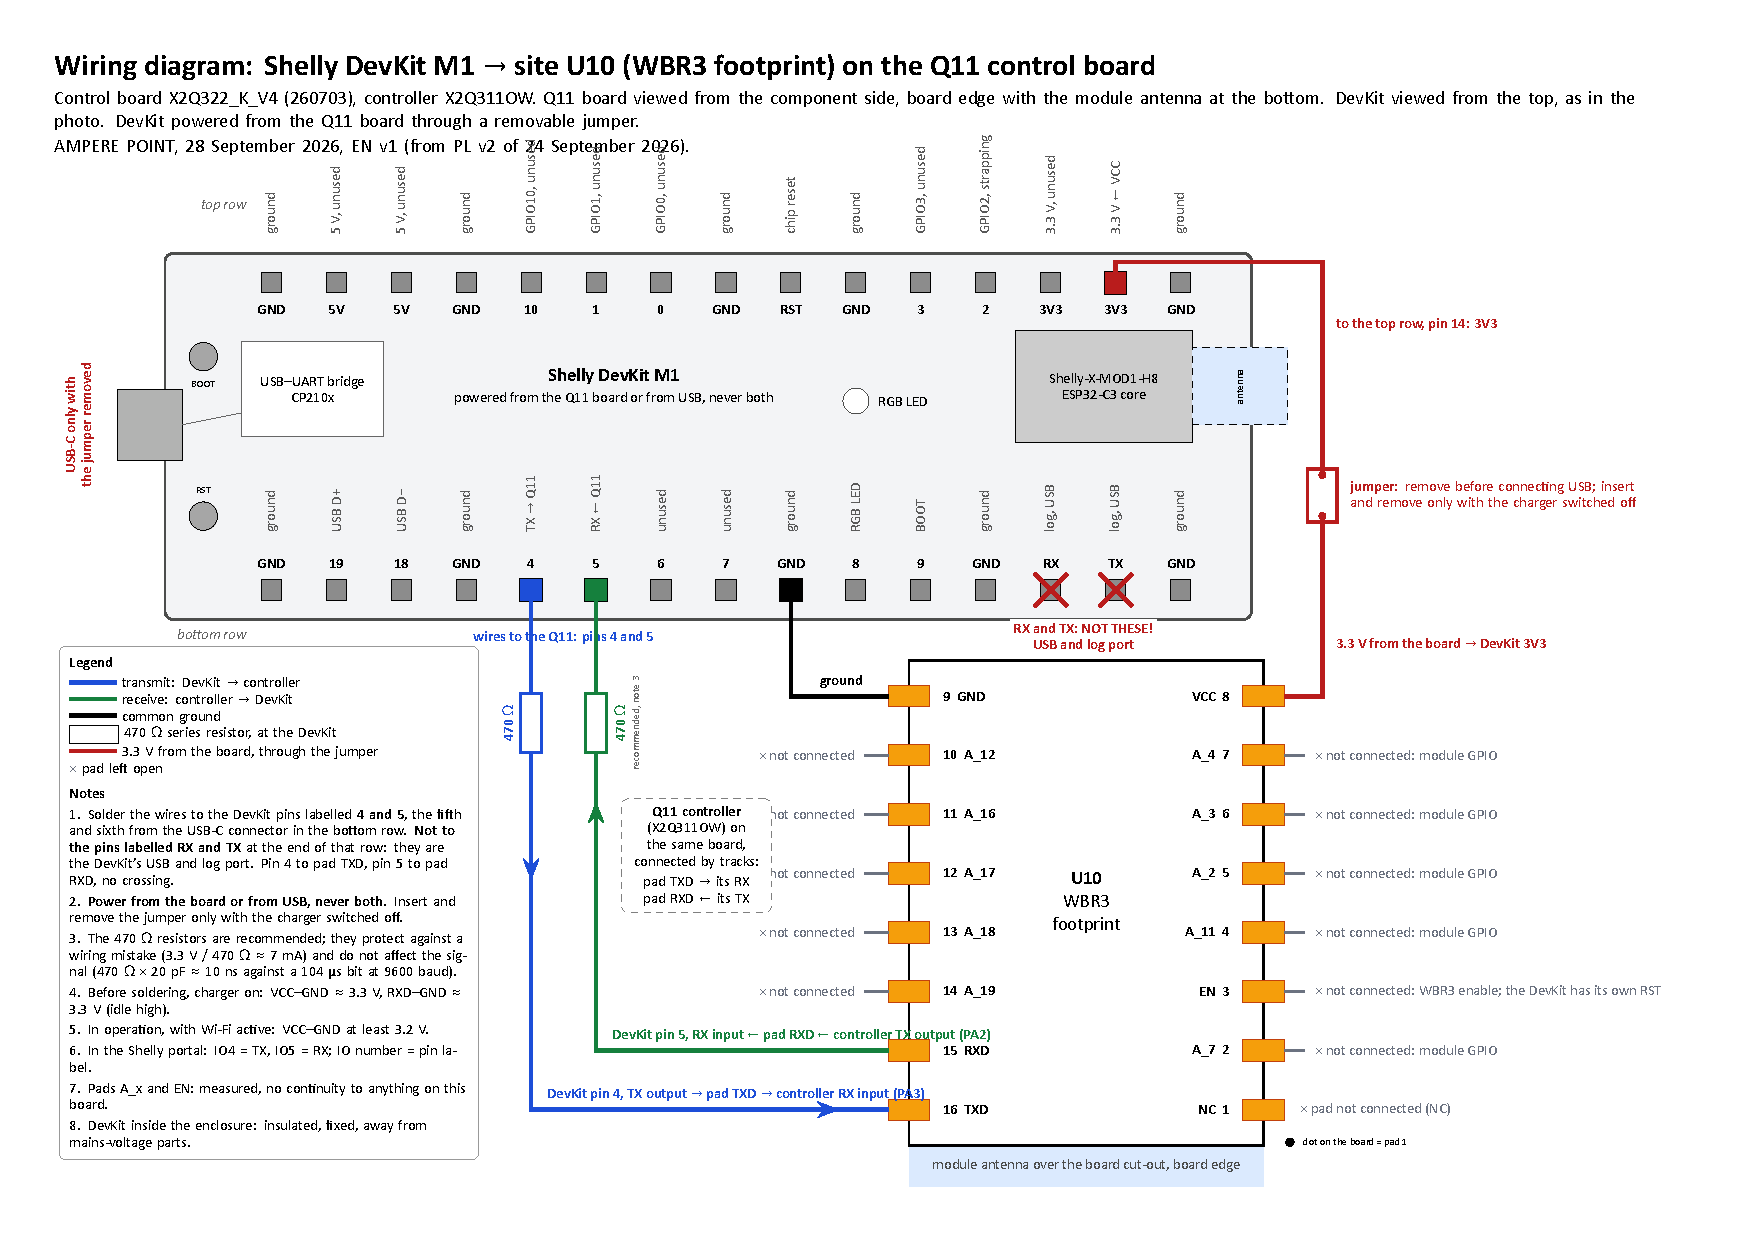
\includegraphics[width=\textwidth]{schematic_wiring_DevKit_Q11_EN.pdf}
\caption{Wiring of the prototype (full-size PDF attached, page 2 shows every pad of U10).}
\label{fig:wiring}
\end{figure}

\begin{figure}[H]
\centering
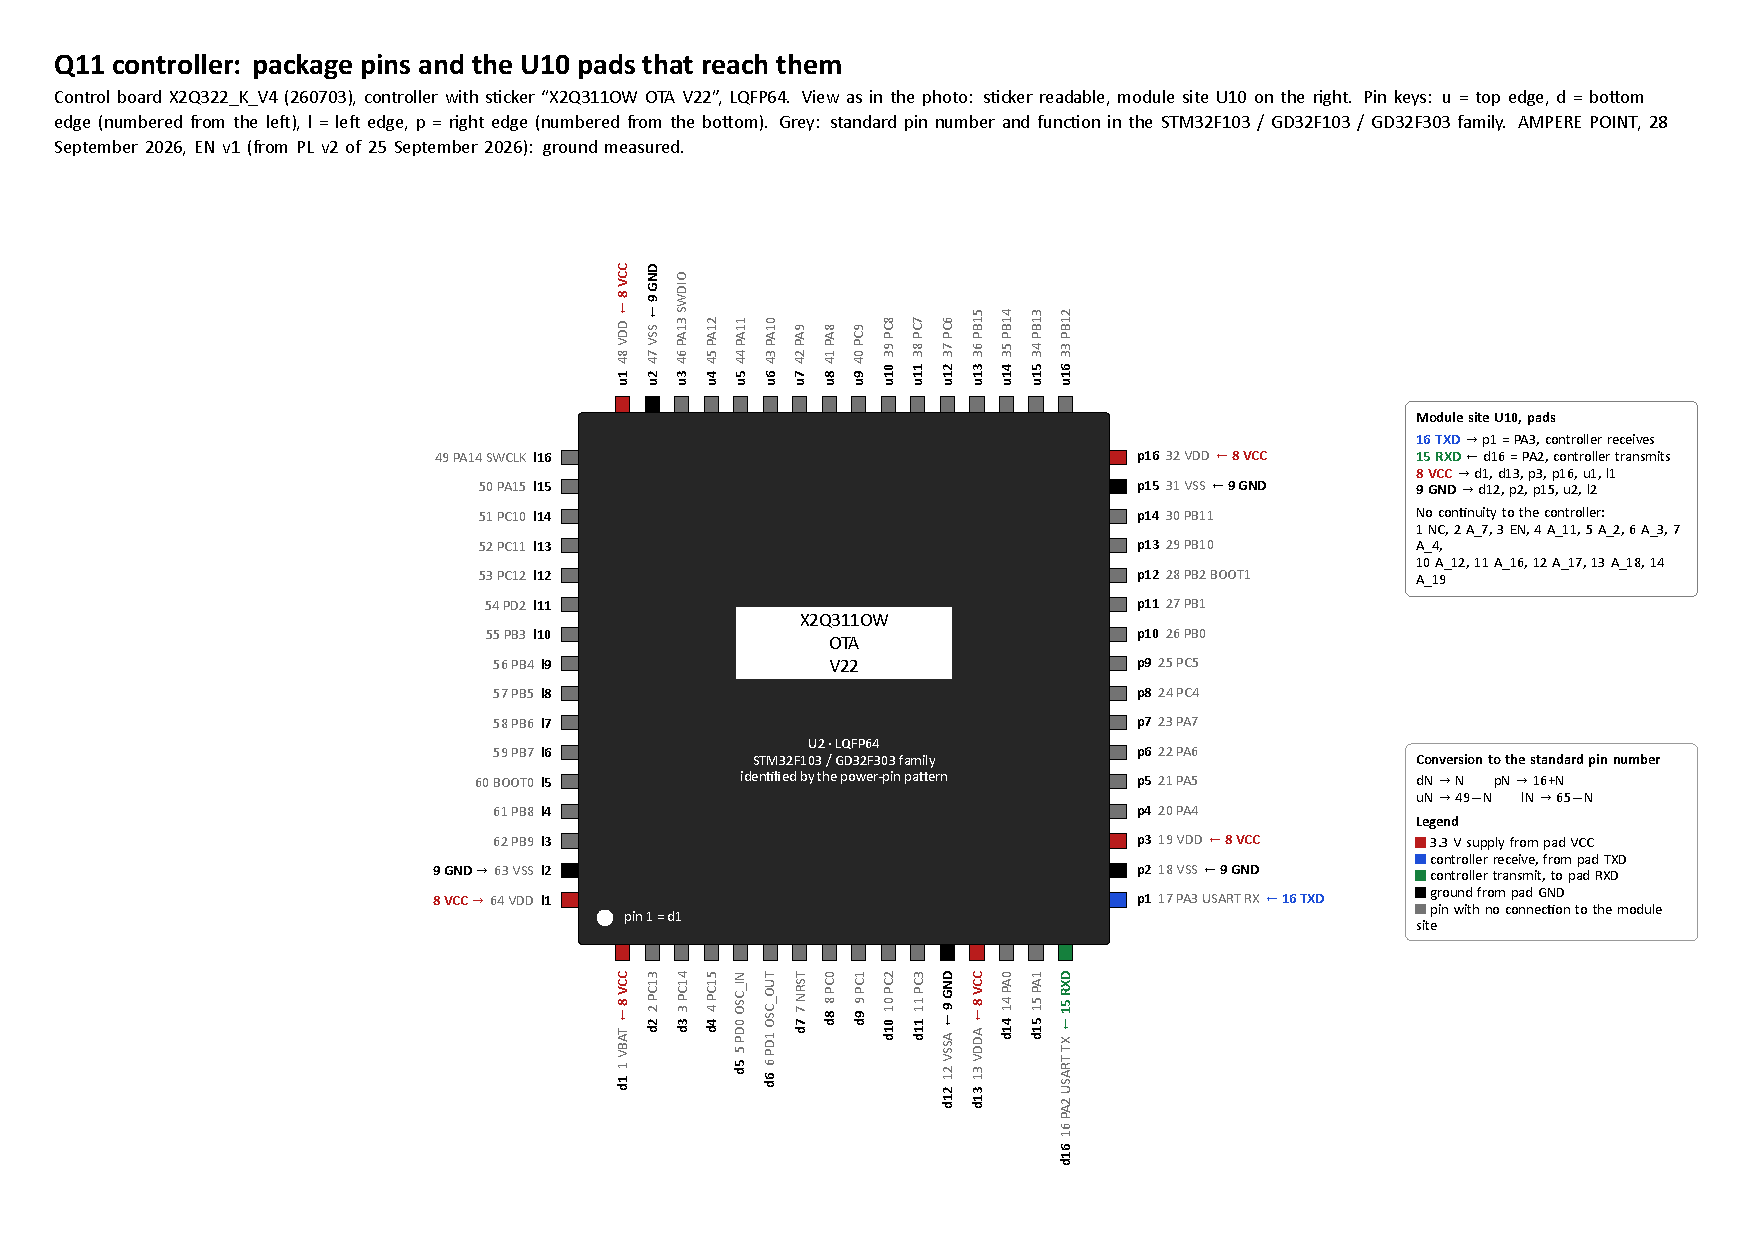
\includegraphics[width=\textwidth]{schematic_Q11_MCU_pins_EN.pdf}
\caption{Controller pins with the U10 pads that reach them (full-size PDF attached).}
\label{fig:mcu}
\end{figure}

\section{Serial protocol as observed on the wire}

\subsection{Physical layer and frame format}

9600~baud, 8 data bits, no parity, 1 stop bit, 3.3~V levels. Tuya MCU serial protocol: \hx{55 AA} $|$ version $|$ command $|$ length (2 bytes, big-endian) $|$ data $|$ checksum (sum of all preceding bytes modulo 256). The controller sends version \hx{03}; the module sends version \hx{00}. The Shelly firmware implements this protocol natively (component ``Tuya MCU''); AmperePoint wrote no protocol code.

\subsection{Start-up handshake}

Captured on 25 September 2026 at 11:51, when the module re-initialised after a configuration upload (the controller stayed powered):

\begin{longtable}{>{\raggedright\arraybackslash}p{1.6cm}>{\raggedright\arraybackslash}p{2.3cm}>{\raggedright\arraybackslash}p{4.1cm}>{\raggedright\arraybackslash}p{7.7cm}}
\toprule
\rowcolor{aphead}\textbf{Time} & \textbf{Direction} & \textbf{Frame (cmd, data)} & \textbf{Meaning} \\
\midrule\endhead
\bottomrule\endfoot
11:51:08 & controller \ra\ module & \hx{0x24} & controller asks for the Wi-Fi signal strength \\
11:51:08 & module \ra\ controller & \hx{0x24 [C7]} & answer: $-57$~dBm \\
11:51:09 & module \ra\ controller & \hx{0x00} & heartbeat \\
11:51:09 & controller \ra\ module & \hx{0x00 [01]} & heartbeat reply, \hx{01} = controller already running (not a fresh boot) \\
11:51:14 & module \ra\ controller & \hx{0x03 [04]} & Wi-Fi status 4 (connected to the cloud, in Tuya terms) \\
11:51:14 & controller \ra\ module & \hx{0x03} & acknowledged \\
11:51:14 & module \ra\ controller & \hx{0x08} & query all data points \\
11:51:16--17 & controller \ra\ module & 12 $\times$ \hx{0x07} & data point reports, in this order: 3, 4, 6, 7, 8, 9, 10, 14, 18, 19, 24, 13 \\
11:51:16 & controller \ra\ module & \hx{0x1C} & controller asks for the time \\
11:51:17 & module \ra\ controller & \hx{0x1C [01 1A 09 19 0B 33 12 05]} & valid, 2026-09-25 11:51:18, weekday 5 \\
\end{longtable}

The product-information exchange (commands \hx{0x01} and \hx{0x02}) happens before the debug log is reachable over Wi-Fi and was not captured; see question~2.

\subsection{Routine traffic}

\begin{itemize}
\item Module \ra\ controller: heartbeat \hx{0x00} every 15~s; Wi-Fi status \hx{0x03 [04]} every 30~s. The controller answers both.
\item Controller \ra\ module: time request \hx{0x1C} and signal-strength request \hx{0x24}, each at irregular intervals of about 10--45~s. The module answers the time request only after it has synchronised its clock (NTP); before that it sends \hx{01 00 00 00 00 00 00 00} (flag ``valid'' with a zero date). AmperePoint therefore provides a local NTP server when the charger is used without Internet.
\item Controller \ra\ module, unsolicited \hx{0x07} reports: temperature (DP~24) on every change, connection state (DP~13) on every change of the control-pilot state, current limit (DP~4) and switch (DP~18) after each write, session energy (DP~25) once at the end of a session.
\end{itemize}

\subsection{Write behaviour}

On a write (\hx{0x06}) the controller first reports the \textbf{old} value, then the \textbf{new} value about one second later. Example, current limit 12~A \ra\ 10~A, 25 September 2026:

\begin{longtable}{>{\raggedright\arraybackslash}p{1.6cm}>{\raggedright\arraybackslash}p{2.5cm}>{\raggedright\arraybackslash}p{6.3cm}>{\raggedright\arraybackslash}p{5.4cm}}
\toprule
\rowcolor{aphead}\textbf{Time} & \textbf{Direction} & \textbf{Complete frame} & \textbf{Meaning} \\
\midrule\endhead
\bottomrule\endfoot
11:56:48 & module \ra\ controller & \hx{55 AA 00 06 00 08 04 02 00 04 00 00 00 0A 21} & set DP~4 (value type, 4 bytes) = 10 \\
11:56:49 & controller \ra\ module & \hx{55 AA 03 07 00 08 04 02 00 04 00 00 00 0C 27} & report DP~4 = 12 (still the old value) \\
11:56:50 & controller \ra\ module & \hx{55 AA 03 07 00 08 04 02 00 04 00 00 00 0A 25} & report DP~4 = 10 (accepted) \\
10:52:37 & module \ra\ controller & \hx{55 AA 00 06 00 05 12 01 00 01 01 1F} & set DP~18 (bool) = 1, charging enabled \\
10:52:38 & controller \ra\ module & \hx{55 AA 03 07 00 05 12 01 00 01 01 23} & report DP~18 = 1 \\
-- & controller \ra\ module & \hx{55 AA 03 00 00 01 01 04} & heartbeat reply, for reference \\
\end{longtable}

Values 8, 10, 12, 14 and 16~A were written and confirmed by the controller in the same way.

\section{Data points}

\subsection{Three layers}

The controller sends its data-point reports on the wire regardless of which module is listening; the Shelly module receives every frame exactly as the WBR3 did. What differs is where the meaning of a data point is defined: with the WBR3 it is the product definition in the Tuya cloud, with the Shelly module it is the product configuration written by AmperePoint. The log confirms that the Shelly module registers every reported data point, including those that are not declared in the product configuration (log entries such as \texttt{add int 24}, \texttt{add enum 13}, \texttt{add raw 19}).

\begin{longtable}{>{\raggedright\arraybackslash}p{6.2cm}>{\raggedright\arraybackslash}p{3.0cm}>{\raggedright\arraybackslash}p{6.9cm}}
\toprule
\rowcolor{aphead}\textbf{Layer} & \textbf{Data points} & \textbf{Defined by} \\
\midrule\endhead
\bottomrule\endfoot
Received and stored by the module & all that the controller sends: 13 different IDs seen & the controller firmware \\
Declared in the Shelly product, available to the service script & 7 (1, 3, 4, 6, 7, 8, 18) & AmperePoint, in the portal \\
Exposed as fields (app, local API, MQTT) & 6 fields & AmperePoint, in the service script \\
\end{longtable}

Enumerations travel on the wire as an index byte; the names exist only in the product definition. The Shelly product uses the same order as the Tuya definition (question~7 asks for confirmation).

\subsection{Comparison: Tuya product definition, controller behaviour, Shelly product}

Definition taken from the Tuya product \emph{Ampere Point Q11 PRO} (17 data points). ``Reported'' = seen in the module log on 25 September 2026: \textbf{dump} = in the answer to the query \hx{0x08}, \textbf{spont.} = sent by the controller on its own, \textbf{never} = not seen in any frame.

\begin{longtable}{>{\raggedright\arraybackslash}p{0.7cm}>{\raggedright\arraybackslash}p{3.1cm}>{\raggedright\arraybackslash}p{3.6cm}>{\raggedright\arraybackslash}p{0.9cm}>{\raggedright\arraybackslash}p{3.2cm}>{\raggedright\arraybackslash}p{3.8cm}}
\toprule
\rowcolor{aphead}\textbf{DP} & \textbf{Tuya code} & \textbf{Type, unit, encoding} & \textbf{R/W} & \textbf{Reported by controller} & \textbf{In the Shelly product} \\
\midrule\endhead
\bottomrule\endfoot
1 & forward\_\allowbreak energy\_\allowbreak total & value, kWh, scale 2 (\hx{123456} = 1234.56~kWh) & R & \no\ never (not in dump, not spont.) & declared, meant for the lifetime counter; stays at 0 because nothing arrives. Question~4 \\
3 & work\_state & enum, 8 states: 0 free, 1 insert, 2 free\_fault, 3 wait, 4 charging, 5 pause, 6 end, 7 fault & R & \ok\ dump; values 0 and 3 seen & \ok\ field ``mode'', index translated to name \\
4 & charge\_cur\_set & value, A, 6--32 & RW & \ok\ dump; writes 8/10/12/14/16 confirmed & \ok\ field ``current limit'', limited to 6--16~A for the Q11 \\
6, 7, 8 & phase\_a / b / c & raw, 7 bytes: voltage 2~B $\times$0.1~V, current 3~B $\times$0.001~A, power 2~B in W & R & \ok\ dump; 226--228~V seen while the contactor was closed; current and power not yet seen under load & \ok\ decoded in the script into the ``phase info'' field \\
9 & power\_total & value, kW, scale 3 & R & \ok\ dump; 0 & \half\ script sums the phases instead \\
10 & fault & bitmap, 17 bits: ov\_cr, ov2\_cr\_fault, ov\_vol, undervoltage\_alarm, contactor\_adhesion, contactor\_fault, earth\_fault, meter\_hardware\_alarm, scram\_fault, cp\_fault, meter\_commu\_fault, card\_reader\_fault, cir\_short\_fault, adhesion\_fault, self\_test\_alarm, leakagecurr\_alarm, ov\_Temp\_fault & R & \ok\ dump; 0 & \half\ received, not yet exposed as a field \\
13 & connection\_state & enum, 7: 0 12V, 1 12V\_pwm, 2 9V, 3 9V\_pwm, 4 6V, 5 6V\_pwm, 6 error & R & \ok\ dump + spont.; values 0, 2, 4 seen & \half\ received, not yet exposed \\
14 & work\_mode & enum, 3: 0 charge\_now, 1 charge\_energy, 2 charge\_schedule & RW & \ok\ dump; 0 & \half\ received, not yet exposed \\
17 & energy\_charge & value, kWh, 1--200 & RW & \no\ never & not declared. Question~4 \\
18 & switch & bool & RW & \ok\ dump + spont. after write & \ok\ field ``state'' \\
19 & local\_timer & raw, 2 bytes: start hour, end hour & RW & \ok\ dump; \hx{00 00} & \half\ received, not yet exposed \\
23 & system\_version & string & R & \no\ never & not declared. Question~4 \\
24 & temp\_current & value, °C, $-40$--200 & R & \ok\ dump + spont. on change; 18--20~°C & \half\ received, not yet exposed \\
25 & charge\_\allowbreak energy\_\allowbreak once & value, kWh, scale 2 & R & \half\ once: value 0, in one frame together with DP~18 = 0 & \half\ session energy is currently computed in the script; will use DP~25 \\
33 & mode\_set & raw & RW & \no\ never & not declared. Question~5 \\
\end{longtable}

The dump answering \hx{0x08} contains 12 data points in this order: 3, 4, 6, 7, 8, 9, 10, 14, 18, 19, 24, 13. Data points 1, 17, 23 and 33 are absent from the dump and were never sent on their own.

\section{Test results}

\begin{longtable}{>{\raggedright\arraybackslash}p{4.2cm}>{\raggedright\arraybackslash}p{1.7cm}>{\raggedright\arraybackslash}p{10.1cm}}
\toprule
\rowcolor{aphead}\textbf{Test} & \textbf{Result} & \textbf{Details} \\
\midrule\endhead
\bottomrule\endfoot
Communication with the controller & \ok & Tuya MCU protocol, 9600 8N1; heartbeat answered; data points reported; no controller firmware change \\
Pads used by the board & \ok & only VCC, GND, RXD, TXD; twelve pads open \\
Module powered from the board & \ok & 3.3~V from the board regulator; no brown-out during the tests \\
Charging on/off from the module & \ok & DP~18 written, confirmed by the controller within 1~s \\
Current limit from the module & \ok & 8, 10, 12, 14, 16~A written and confirmed \\
Status read-out & \ok & work state, connection state, temperature, fault bits, work mode, timer window, phase voltages \\
Time delivered to the controller & \ok & \hx{0x1C} answered with the correct local time once the module has NTP; a local NTP server is used off-line \\
Wi-Fi status to the controller & \ok & \hx{0x03 [04]} every 30~s; the charger display shows the network icon \\
Operation without any cloud & \ok & the Shelly cloud disabled; module controlled over the local network (HTTP, WebSocket, MQTT) and over Bluetooth \\
Local integration layer & \ok & see below \\
Charging under load & \half & a vehicle simulator was used for the control-pilot states; a full session with current flowing is still to be done \\
Controller firmware update through the module & \no\ not tested & see question~9 \\
Wi-Fi reset from the charger menu & \no\ not tested & see question~8 \\
\end{longtable}

\begin{apbox}[Local integration layer (middleware), for information]
The Shelly module exposes a local API (HTTP, WebSocket, MQTT). On top of it AmperePoint runs a small software layer outside the charger: an MQTT broker, a local NTP server and a bridge that presents the Q11 to a charging back-end as an OCPP~1.6J charge point (registration, status, remote start, current limit via charging profile, meter values). All of this was tested against a local test server. It lives on a computer or server, not in the charger, and \textbf{needs nothing from the controller firmware}. It is mentioned here only so that the whole picture is visible.
\end{apbox}

\section{Open questions for the factory}

\begin{enumerate}
\item \textbf{Controller part number.} Which microcontroller is under the sticker ``X2Q311OW OTA V22'' (STM32F103xx, GD32F103xx, GD32F303xx, other), and what is its flash size?
\item \textbf{Product information frame.} What does the controller answer to the product query (\hx{0x01}): product key \texttt{p}, firmware version \texttt{v}, module working mode \texttt{m}? Which Tuya MCU SDK / protocol version does the firmware implement? We could not capture this exchange because it happens before the module log is reachable.
\item \textbf{Unconnected pads.} Twelve pads of U10 (NC, A\_7, EN, A\_11, A\_2, A\_3, A\_4, A\_12, A\_16, A\_17, A\_18, A\_19) show no continuity to anything. Please confirm from the schematic that the board uses only VCC, GND, RXD and TXD of the module, and that the firmware does not expect any signal on the other pads (for example EN, or a reset line).
\item \textbf{Data points never reported.} DP~1 (forward\_energy\_total), DP~17 (energy\_charge), DP~23 (system\_version) and DP~33 (mode\_set) were not in the dump and were never sent on their own. Under which conditions does the controller report each of them? DP~25 (charge\_energy\_once) was sent once, with value 0, together with DP~18 = 0: is that the end-of-session report?
\item \textbf{DP~33 mode\_set.} What is the byte format and the meaning of this raw data point?
\item \textbf{DP~8.} In the export of \texttt{Q21\_11kW\_with\_OTA} DP~8 is named \texttt{charger\_events}, in the \emph{Q11 PRO} definition it is \texttt{phase\_c}. Our unit sends DP~8 as a 7-byte raw value in the same format as DP~6 and DP~7. Which definition does the shipped firmware follow, and does the format differ between firmware versions?
\item \textbf{Enumeration order.} Please confirm the index order of DP~3, DP~13 and DP~14 as listed in the table above.
\item \textbf{Wi-Fi status and pairing.} Which Wi-Fi status values (\hx{0x03}, 0--7) does the controller use, and for what (display icon, behaviour)? What does the charger's menu item for network reset / pairing send to the module (\hx{0x04} or \hx{0x05})?
\item \textbf{Controller firmware update through the module.} Does the controller support the Tuya MCU update commands (\hx{0x0A} start, \hx{0x0B} packet transfer)? Which file format is uploaded to the Tuya platform for the MCU OTA (plain binary?), and could the same file be provided to AmperePoint so that the Shelly module, which implements the same update commands, can update the controller? Does the bootloader tolerate an interrupted update?
\item \textbf{Time.} The controller asks for the time (\hx{0x1C}) every 10--45~s. What does it use the time for (timer window DP~19, display, session records), and what happens if the module never supplies a valid time?
\item \textbf{Behaviour when the module is silent.} The controller kept working normally when the module sent nothing for a day (miswired prototype). Is there any timeout on the heartbeat or on the Wi-Fi status that changes the controller's behaviour?
\end{enumerate}

\section{Attachments}

\begin{itemize}
\item \texttt{ShellyX\_module\_X1\_datasheet\_v14.pdf}: datasheet of the target module (Shelly).
\item \texttt{schematic\_wiring\_DevKit\_Q11\_EN.pdf}: wiring of the prototype and function of every pad of U10.
\item \texttt{schematic\_Q11\_MCU\_pins\_EN.pdf}: controller pins with the U10 pads that reach them.
\item Frame-level logs of the module (25 September 2026) are available on request.
\end{itemize}

{\color{apmuted}\small AMPERE POINT — R\&D · www.amperepoint.pl · Prepared on 28 September 2026 from measurements on a Q11 unit, the module debug log and the Tuya product definitions.}

\end{document}
